\documentclass[12pt,a4paper]{article}

\usepackage[utf8]{inputenc}
\usepackage[portuguese]{babel}
\usepackage[T1]{fontenc}
\usepackage[left=2.5cm,right=2.5cm,top=2cm,bottom=2cm]{geometry}
%\usepackage{fancyhdr}
%\pagestyle{fancy}
\usepackage{graphicx}
\usepackage{color}
\usepackage{indentfirst}
\usepackage{wrapfig}
\usepackage{lipsum}
\usepackage{setspace}
\usepackage{adjustbox}
\usepackage{minted}
\usepackage{amsmath}
\bibliographystyle{unsrtnat}
\usepackage[numbers,sort&compress]{natbib}
\usepackage{breakcites}
\usepackage[breaklinks=true]{hyperref}
\usepackage{hyperref}

\usepackage{microtype} % Improves typography
\usepackage{gfsdidot} % Use the GFS Didot font: http://www.tug.dk/FontCatalogue/gfsdidot/


% Create a new command for the horizontal rule in the document which allows thickness specification
\makeatletter
\def\vhrulefill#1{\leavevmode\leaders\hrule\@height#1\hfill \kern\z@}
\makeatother
\parindent 1cm

 \renewcommand{\rmdefault}{phv} % Arial
 \renewcommand{\sfdefault}{phv} % Arial

\title{Relatório PIBIC Daniel Benvenutti}
%\author{}

\thispagestyle{empty}

\begin{document}


\begin{wrapfigure}[2]{l}{7cm}

\includegraphics[scale=0.111]{logo-documentos.png}
\end{wrapfigure}



\noindent 
\begin{flushright}
\begin{scriptsize}
Francisco Rouxinol \\
Instituto de Física Gleb Watghin\\
Rua Sergio Buarque de Holanda, 777\\
13083-859, Campinas, SP \\
e-mail: rouxinol@unicamp.br\\
tel: +55(19)3521-5462\\
% \hspace{-0.5cm} 
\vhrulefill{1pt} \\ % 
\end{scriptsize}
\end{flushright}

% \singlespacing %Para um espaçamento simples
% \onehalfspacing %Para um espaçamento de 1,5
%\doublespacing %Para um espaçamento duplo 

% $ $\\


% \singlespacing %Para um espaçamento simples
% \large 
\begin{flushleft}
\textbf{Projeto Principal}: “Algoritmo quântico de busca de Grover e de fatoração de Shor: implementação da simulação em computadores clássicos e quânticos”\\
\textbf{Grande Área de conhecimento:} Ciências Exatas e da Terra\\
% \textbf{Grande Área de conhecimento: }Ciências Exatas e da Terra\\
\textbf{Área de Conhecimento:} Física\\
\textbf{Subárea de Conhecimento: }Física da Matéria Condensada\\
\textbf{Aluno(a):} Daniel Benvenutti\\
\textbf{Orientador: }Francisco Rouxinol\\
\textbf{Instituição:} Instituto de Física Gleb Wataghin, UNICAMP\\
\textbf{Palavras chaves:} Eletrodinâmica Quântica, Computação Quântica e Informação\\
\textbf{Referente:} Primeiro Relatório
\end{flushleft}


%  \singlespacing %Para um espaçamento simples
\abstract{\textbf{Resumo do projeto original:} Nós apresentamos um projeto de pesquisa focado no desenvolvimento pelo aluno de um conjunto de ferramentas para simular algoritmos quânticos em computadores clássicos e quânticos. Serão tratados e discutidos os conceitos básicos de computação quântica e mecânica quântica, como também a implementação de portas quânticas e o algoritmo de busca de Grover e de fatoração de Shor. Com a implementação deste projeto é esperado que importantes conceitos de quântica, como medida, funções de onda de muitos corpos, e momento angular, sejam aprofundados como também o estudo de importantes tópicos avançados em física e engenharia. }

%  \singlespacing %Para um espaçamento simples


\section{Introdução}
O \textit{objetivo do projeto }era levar o estudante a pensar profundamente em como um computador baseado em lógica quântica funciona. Utilizando um conjunto de ferramentes computacionais o estudante deveria desenvolver em um computador clássico um conjunto de portas lógicas quânticas e simular diversos algorítimos quânticos (i.e. Grover\cite{Grover1996ASearch}, Shor\cite{Shor1997Polynomial-timeComputer}, etc) e testar em computadores quânticos disponíveis \textit{online} estes sistemas. \textit{Em longo prazo}, este projeto está preparando o aluno para entender de forma mais clara importantes  tópicos modernos de computação quântica, física, e programação em sistemas quânticos - preparando o caminho  para o desenvolvimento de projetos mais avançados neste fascinante campo de pesquisa.

Um importante aspecto do projeto foi o desenvolvimento dos vetores de estado e portas lógicas utilizando as bibliotecas  Scipy e Sympy existentes na linguagem Python \cite{Rossum2011}, como na experiência de aplicar e desenvolver conceitos de física quântica numa das suas aplicações práticas, \textit{a computação quântica}. 

Durante os primeiros 3 bimestres, trabalhamos na preparação das diversas portas quânticas necessárias para execução dos algorítimos estudados neste projeto.  Para escrever os programas utilizamos ambiente de desenvolvimento interativo Jupyter \cite{Kluyver2016} com a linguagem de programação Python \cite{Rossum2011}. Foram desenvolvidos os algorítimos para a \textit{inicialização do sistema}, a \textit{operação de portas quânticas}, e a \textit{medição dos estado}. 

Nos 3 bimestres finais, trabalhamos na implementação da execução dos algorítimos e na aprendizagem da utilização dos computadores quânticos da IBM \cite{IBM2019IBMExperience}. Terminamos o trabalho comparando os resultados da simulação dos algorítimos quânticos rodados em computadores clássico com os resultados das simulações dos algorítimos em computadores quânticos da IBM. 



\section{Atividades Principais}

De forma resumida, durante o projeto,trabalhamos nas quatro etapas do cronograma. Inicialmente desenvolvemos os registradores de N-qubits. Cada registrador guardava a informação do estado composto por 3 sistemas de dois níveis (qubits), descrito por um único estado quântico conjunto $|\psi\rangle$.  Utilizando estes vetores, preparamos algorítimos para preparar o sistema de interesse no estado de desejado. 

Na segunda etapa, desenvolvemos funções que simulam uma porta quântica (análogo a uma porta lógica), necessárias para operar os qubits. Utilizando os elementos dos vetores de estado e a portas lógicas, a probabilidade de medir um determinado valor pode ser determinado, simulando-se uma medida no sistema quântico. 

Com estas funções e algorítimos programados, foram preparados os algorítimos de Groover de busca e Shor de fatoração de números inteiros. Ambos funcionaram como esperado. O de Groover amplificando a probabilidade do estado buscado até ele se destacar entre os outros. E o de Shor obtendo como saída o período de uma função do algoritmo que é o passo do algoritmo para fatorar o número realizado no computador quântico.

Na última implementamos os algorítimos Groover de busca e Shor de fatoração de números inteiros no computador quântico da IBM e comparamos com os resultados obtidos em nosso programa.

Nas próximas seções descrevemos em mais detalhes as etapas desenvolvidas neste período. Também fornecemos o código utilizando nesta etapa na plataforma GitHub no endereço: \url{https://github.com/Danielgb23/ic_comp_quantica}
% {https://github.com/Danielgb23/ic_comp_quantica/blob/master/caderno_qiskit_comp_real.ipynb}

\subsection{Registrador Quântico}
A primeira parte do projeto e construir o simulador. Para simular o estado de $N$ qubits precisamos de um vetor de  $2^{N}$ elementos.
Por exemplo, um vetor de 3 qubits com 8 elementos:

$${ \psi=[0, 0, 0, 0, 0, 0, 0, 0]}$$

Cada estado nesse vetor representa uma combinação das medidas possíveis dos qubits. O primeiro estado é $|000\rangle$ o segundo é $|001\rangle$, o terceiro é $|010\rangle$ e assim por diante até o oitavo, $|111\rangle$.

Em seguida precisamos poder medir esse estado quântico. Uma medida é representada por por uma escolha aleatória do computador levando como pesos probabilísticos os elementos do vetor de estado com maior módulo complexo ao quadrado.

$${[0, 1, 0, 0, 0, 0, 0, 0]}$$

Por exemplo, o segundo elemento do vetor acima tem 100\% de chance de ser medida.

$${[0.5, 0.5, 0.5, 0.5, 0, 0, 0, 0]}$$

Já neste caso, temos $|0.5|^{2}=1/4$ de chance de ser medido no primeiro, segundo, terceiro ou quarto estados.


\subsection{Portas quânticas}
\subsubsection{Porta de Hadamard}

\begin{figure}[h]
    \centering
    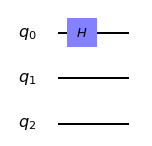
\includegraphics{hadamard_gate.png}
        \caption{Porta de Hadamard}
    \label{fig:hgate}
\end{figure}

Uma das portas quânticas mais importantes é a \textit{Porta de Hadamard}, $H$. Ela é extremamente interessante, pois coloca um qubit em uma superposição de dois estados. Por exemplo, o código:

\begin{minted}[mathescape, linenos]{python}
qubit=[1,0] # estado inicial do qubit
qubit=hadamard(qubit, 1, 1) # hadamard no primeiro qubit
print(qubit)
\end{minted}[mathescape, linenos]{python}
retorna

$$[0.707106781186547, 0.707106781186547]= [1/\sqrt{2},1/\sqrt{2}]= |\psi\rangle=\frac{1}{\sqrt{2}}\left(|0\rangle+|1\rangle\right)$$

\subsubsection{Porta de Fase}
Outra importante porta é a \textit{Porta de Fase}, $S$.  Ela muda a fase complexa do elemento do vetor que descreve o qubit.

\begin{equation}
S=\left| \begin{array}{cc} 1 & 0 \\ 0 & e^{i\theta} \end{array}  \right|  
% \left| \begin{array}{cc} x_{11} & x_{12} \\ x_{21} & x_{22} \end{array} \right|
\end{equation}

Então se usarmos uma dessas portas:

\begin{minted}[mathescape, linenos]{python}
qubit=[0,1] # estado inicial do qubit
qubit=muda_fase(qubit, 1, math.pi/2, 1)
print(qubit)
medir_n(qubit, 100, 1)
\end{minted}[mathescape, linenos]{python}

obtemos:

$$|\psi\rangle=[0,\, 0 + 1.0i]$$

Que tem um número imaginário puro no segundo elemento do vetor, devido a mudança de fase de $\pi/2$. 
% já que ele é $|1\rangle$ no caso de um único qubit e que a fase da nossa mudança é $\pi/2$.

\subsubsection{Porta CNOT}


\begin{figure}[h]
    \centering
    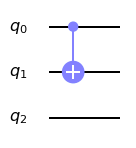
\includegraphics{cnot_gate.png}
    \label{fig:cnotgate}
        \caption{Porta CNOT}
\end{figure}

 Portões CNOT são portas quânticas NOT (ou NÃO) controladas e funcionam da seguinte maneira: Há um qubit controlador e um qubit que sofre a operação NOT. Se e somente se o qubit controlador é $|1\rangle$ que o outro qubit é invertido de $|1\rangle$ para $|0\rangle$ ou de $|0\rangle$ para $|1\rangle$. Se o controlador for $|0\rangle$ o controlado mantém o seu estado. O qubit controlador não é alterado. Com essa porta podemos fazer o estado de emaranhamento quântico:
 
 \begin{minted}[mathescape, linenos]{python}
Psi=[0]*8 # estado inicial

seta_base(Psi,0)
#hadamard no segundo qubit para coloca-lo numa superposição
Psi=hadamard(Psi, 2, 3)  

#CNOT para emaranhar os qubits
Psi=cnot3(Psi, 3)

print(Psi)
medir_n(Psi, 1000, 3)
 \end{minted}[mathescape, linenos]{python}

$$|\psi\rangle = [0.71, 0, 0, 0.71, 0, 0, 0, 0]$$

% 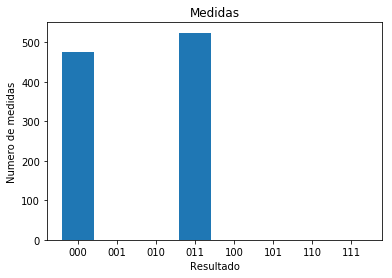
\includegraphics[]{relatorio-superposicao.png}
\begin{figure}
    \centering
    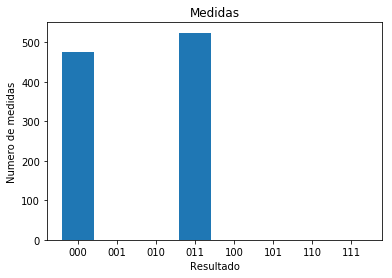
\includegraphics[width=0.8\textwidth]{relatorio-superposicao.png}
    \caption{Histograma com valores obtidos para 1000 medidas de uma Porta CNOT }
    \label{fig:CNOT}
\end{figure}

Obteremos uma superposição entre os dois estados $|000\rangle$ e $|011\rangle$.  Logo, há uma correlação na medida do segundo e terceiro qubit. Se um é medido zero (1) o outro também é, se um é medido 1 o outro também será.




\subsection{Algoritmo de Groover}
O algoritmo de Groover é um algoritmo de busca. Dado um vetor de possíveis respostas,  procuramos neste vetor, um valor específico, que indica qual é a resposta correta. 
Com uma algoritmo normal de varredura em um computador clássico no pior caso temos que verificar todos os $n$ elementos. Já no algoritmo de Groover precisamos de apenas $\sqrt{n}$ buscas.

Apesar disso a nossa lista precisa ser armazenada num oráculo quântico que é um operador que será utilizado nos nossos qubits. O que é o mais difícil.


O algoritmo de Groover funciona usando uma técnica chamada amplificação de amplitude. A fase do elemento do vetor que é a resposta procurado é invertida, e em seguida, com o operador de difusão de Groover é amplificada. Isso é repetido um número ótimo de vezes, o que deixa a resposta correta com uma maior probabilidade de ser medida.

Aqui temos uma execução do código:
\begin{minted}[mathescape, linenos]{python}

Psi=[1,0,0,0,0,0,0,0]

count=1
while count <= 3:    #passa o loop pelo vetor psi
    Psi=hadamard(Psi, count, 3) #hadamard em todos os qubits
    count = count + 1

resposta=6

#blocos do operador de difusao de groover
Psi=bloco_groover(Psi, 3, resposta)
Psi=bloco_groover(Psi, 3, resposta)

print(Psi)
medir_n(Psi, 1000, 3)
\end{minted}[mathescape, linenos]{python}

O vetor resposta encontrado é:


$$|\psi\rangle= [-0.08, -0.08, -0.08, -0.08, -0.08, -0.08, 0.97, -0.08]$$

Onde a amplitude do 7 elemento '110' (6  já que se começa do 0) é $0.97$ enquanto a dos outros é de apenas $-0.08$. É importante lembrar que a probabilidade medida durante o experimento será \(\psi^2\)



% 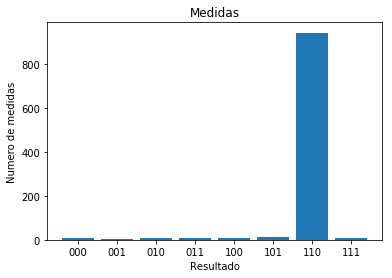
\includegraphics[]{relatorio_groover.png}
\begin{figure}
    \centering
    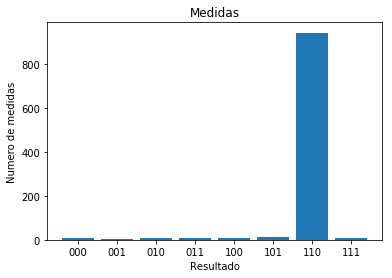
\includegraphics[width=0.8\textwidth]{relatorio_groover.png}
    \caption{Histograma com valores obtidos para 1000 medidas para o algorítimo de Groover }
    \label{fig:Groover}
\end{figure}

Em seguida avaliamos o desempenho da simulação do algoritmo de Groover no meu computador. Abaixo os resultados:

\begin{table}[htb]

\begin{adjustbox}{center}
\begin{tabular}{|l|l|}  
\hline
Qubits  & tempo \\ \hline
1  & 1.20s \\ \hline
2  &  1.15s\\ \hline
3  &   1.36s\\ \hline
4  &  3.51s\\ \hline
5  &  29.33s\\ \hline
6  &   353.69s\\ \hline

\end{tabular}
\end{adjustbox}
\caption{Tempos de simulação para diferentes números de qubits}
\end{table}


Depois o algoritmo de Groover foi executado utilizando-se matrizes esparsas. Que são muito úteis nessas simulações, já que as matrizes dos operadores têm muitos zeros.

\begin{minted}[mathescape, linenos]{python}
    
qubits=input()
resposta=1

Psi=[0]*2**qubits
Psi[0]=1

count=1
while count <= qubits:    #passa o loop pelo vetor psi
        Psi=sp_hadamard(Psi, count, qubits) #hadamard em todos os qubits
        count = count + 1

#blocos do operador de difusao de groover
count=1
   #passa o loop pelo vetor psi
while count <= round(math.pi/4*math.sqrt(2**qubits)): 
        Psi=sp_bloco_groover(Psi, qubits, resposta)
        count = count + 1
print(Psi)
print("done")

\end{minted}[mathescape, linenos]{python}


\begin{table}[htb]
\centering
\begin{adjustbox}{center}
\begin{tabular}{|l|l|}  
\hline
Qubits  & tempo \\ \hline
1  & 0.86s \\ \hline
2  &  0.92s\\ \hline
3  &   0.91s\\ \hline
4  &  0.97s\\ \hline
5  &  1.04s\\ \hline
6  &   1.16s\\ \hline

7  &   1.42s\\ \hline

8  &   2.16s\\ \hline

9  &   5.06s\\ \hline

10  &   19.40s\\ \hline

11 &   105.38s\\ \hline

12 &   626.17s\\ \hline

13 &   353.69s\\ \hline

\end{tabular}
\end{adjustbox}
\caption{Tempos de simulação para diferentes números de qubits utilizando matrizes esparsas}
\end{table}

Nota-se a grande melhoria no desempenho e como é possível utilizar um número muito maior de qubits com o mesmo computador.

\subsection{Algoritmo de Shor}
 O algoritmo de Shor é um algoritmo de fatoração de números inteiros. Um dos seus passos é acelerado se executado em um computador quântico. Abaixo os passos do algoritmo:

Dado um número $C$ que se deseja encontrar os fatores:

\begin{enumerate}

 \item Cheque se $C$ é impar e não é potência de algum inteiro pequeno. Se for um desses encontramos um fator de $C$ e terminamos.

 \item Pegue qualquer inteiro no intervalo $1 < a < C$.

 \item Encontre o $mdc(a, C)$ (maior divisor comum). Se o mdc for maior que 1 por sorte, encotramos ja um fator de C e terminamos.

 \item Encontre o menor inteiro $p$ tal que $a^{p} \equiv 1\, mod\, C$. A expressão  $p \equiv q \, mod\, C$ quer dizer a congruência modular. Ou seja $p-q$ é um inteiro multiplo de C. Isso pode ser escrito também como $p\, mod\, C = q\, mod\, C$.

 \item Se $p$ é impar ou se $p$ é par e $a^{p/2} \equiv -1\, mod\, C$ volte para 2 e escolha um novo $a$.

 \item Os números $P_{\pm} = mdc( a^{p/2} \pm 1, C)$ são fatores não triviais de C.

\end{enumerate}

O computador quântico é responsável pelo 4º passo desse algoritmo. O resto dos passos como encontrar o mínimo divisor comum (mdc) são feitos rapidamente em um computador clássico.

Esse passo se chama encontrar o período pois $f(x)=a^{x} \, mod \, C$ é uma função periódica com período $p$. Dividimos o registrador quântico em duas partes: o registrador $x$ com $L$ qubits iniciado em $|0...0\rangle$ e o $f$ com $M$ qubits iniciado em $|0...01\rangle$:

O quarto passo:


\begin{enumerate}
\item Aplique portas de Hadamard em todos os L qubits do registrador $x$, representado por $H^{\otimes L}$. Isso coloca o registrador $x$ numa superposição de todos os $2^{L}$ estados possíveis

\item Multiplique o registrador $f$ por $a^{x} \, mod \, C$ fazendo com que fique com o valor de $f(x)$.

\item Meça o registrador $f$ (esse passo é opcional)

\item Faça uma transformada de Fourier quântica inversa (IQFT em inglês) no registrador $x$. A IQFT permite encontrar o período da função.

\item Meça a saída $\bar{x}$ de do IQFT (lembrando que temos que ler a saída do IQFT na direção contrária).  Shor provou que $\bar{x}/2^{L}$ é igual a aproximadamente $s/p$ onde $s$ é um inteiro qualquer. Usamos isso para encontrar $p$. Por exemplo $\bar{x}/2^{L} = 0.32 \cong 1/3 = 2/6 = 3/9$ então $p$ é $3, 6, 9, \cdots$ Checamos em seguida esses valores para ver se $a^{p} \equiv 1\, mod\, C$.

\end{enumerate}



\begin{minted}[mathescape, linenos]{python}
# Início do programa
a=2
#psi comeca em |0000001>
qubits=7
psi=[0]*(2**qubits)
seta_base(psi,1)

#coloca em superposicao os bits de L
psi=sp_hadamard(psi, 3, qubits) #hadamard em l0 
psi=sp_hadamard(psi, 2, qubits) #hadamard em l1 
psi=sp_hadamard(psi, 1, qubits) #hadamard em l2 
print "qubits L em superposição"
print psi

#parte de f de x
#multiplica por a se l0=1
psi=shor_fx(psi, 1, a, 15, 3, 4) 
 #multiplica por a^2 se l1=1
psi=shor_fx(psi, 2, a**2, 15, 3, 4)
#multiplica por a^3  se l2=1
psi=shor_fx(psi, 3, a**4, 15, 3, 4) 
# terminado e multiplicando por a^(l2l1l0)

print "-------------------------"
print "matrizes de permutação aplicadas para econtrar f(x)"
print psi

#IQFT transformada de fourier quantica inversa
psi=sp_hadamard(psi, 1, qubits) #hadamard em l2

#mudanca de fase de pi/2 controlada por l2 em l1
psi=sp_Cfase(psi, 2, 1, qubits, math.pi/2) 

#mudanca de fase de pi/4 controlada por l2 em l0
psi=sp_Cfase(psi, 3, 1, qubits, math.pi/4) 

psi=sp_hadamard(psi, 2, qubits) #hadamard em l1

#mudanca de fase de pi/2 controlada por l2 em l1
psi=sp_Cfase(psi, 3, 2, qubits, math.pi/2) 

psi=sp_hadamard(psi, 3, qubits) #hadamard em l0 

print "-------------------------"
print "transformada de fourier quântica inversa aplicada"
print "para encontrar o período da função"
print psi

medir_xbarra_shor(Psi, 1000, 3, 4)
\end{minted}[mathescape, linenos]{python}

% 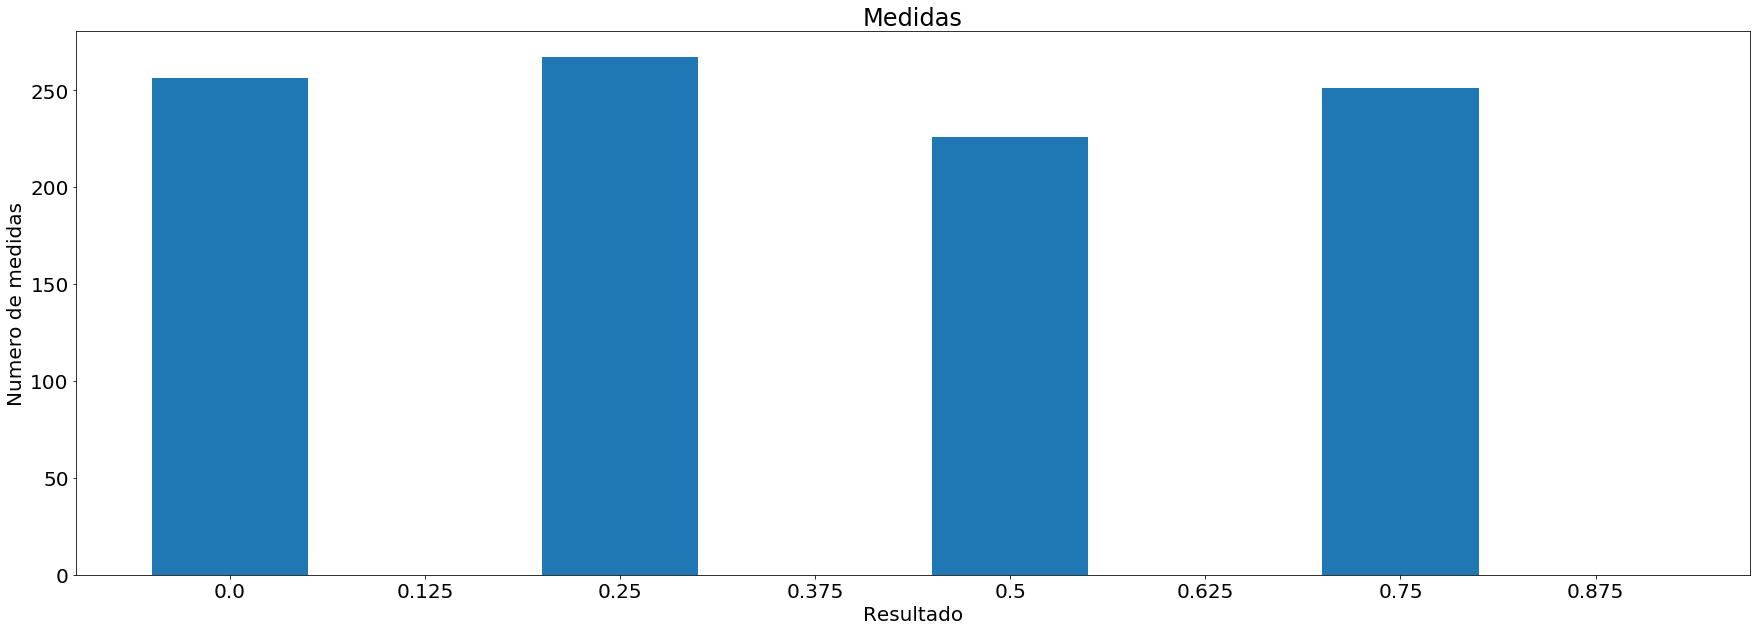
\includegraphics[scale=0.25]{relatorio-shor1.png}

\begin{figure}
    \centering
    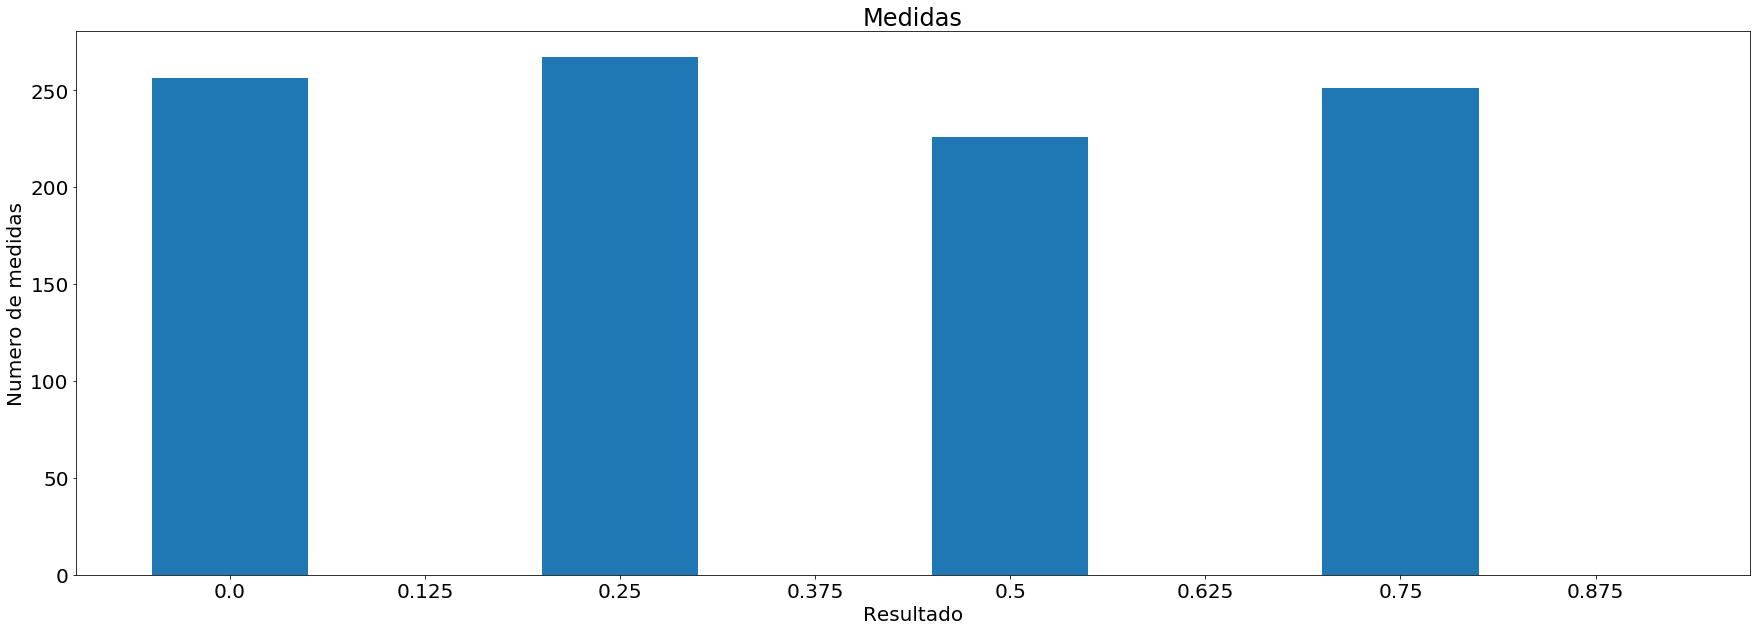
\includegraphics[width=1\textwidth]{relatorio-shor1.png}
    \caption{Histograma com valores obtidos para a aplicação do algoritmo de Shor com 7 qubits fatorando 15 com a=2}
    \label{fig:Shor1}
\end{figure}


Agora medimos o resultado no registrador obtendo vários valores para $\bar{x}/2^{L}$ onde $\bar{x}$ é o valor do registrador $x$ após a aplicação do IQFT com os bits invertidos. Esses valores são a frequência da função e seus harmônicos $s\omega$ onde $s$ é um inteiro. Ou seja obtemos como medida um valor $s/p$ para a medida de $\bar{x}/2^{L}$ onde $s$ é um inteiro qualquer e $p$ é o valor procurado do período para o algoritmo de Shor. Como obtemos quatro valores principais podemos concluir que p=4. Na prática, podemos contar o número de picos principais na medidas de saída. 4 picos equivale a um período de 4 por exemplo. Também podemos usar frações parciais para aproximar o valor desejado a partir das resultados da saída do computador quântico.



Também fizemos simulações do algorítimo de Shor para um número N arbitrário de qubits:

\begin{minted}[mathescape, linenos]{python}
# Inicio do programa
a=10
L=6
M=6
C=21

#psi comeca em |00 ... 01>
qubits=L+M
psi=[0]*(2**qubits)
seta_base(psi,1)


#coloca em superposicao os bits de L
j=1
while j<=L :
    psi=sp_hadamard(psi, j, qubits) #hadamard
    print "had", j
    j = j + 1
    

#parte de f de x
j=1
while j<=L :
#multiplica por a^3  se l2=1 terminado e multiplicando por a^(l2l1l0)
    psi=shor_fx(psi, j, a**(2**(j-1)), C, L, M) 
    print "fx", j
    j = j + 1
    

#IQFT transformada de fourier quantica inversa
i=1

while i <= L:
    
    psi=sp_hadamard(psi, i, qubits) #hadamard em l2 
    #print "hadamard", i
    j=1
    while j <= L-i:
     #mudanca de fase de pi/2 controlada por l2 em l1
        psi=sp_Cfase(psi, i+j, i, qubits, math.pi/(2**j))
        #print i+j, "controls pi/",2**j, "on", i
        j = j + 1
    print "IQFT", i
    i = i + 1
    

print 'terminado'

#plota
Psi=psi.toarray()[0]
medir_xbarra_shor(Psi, 1000, L, M)

\end{minted}[mathescape, linenos]{python}


% 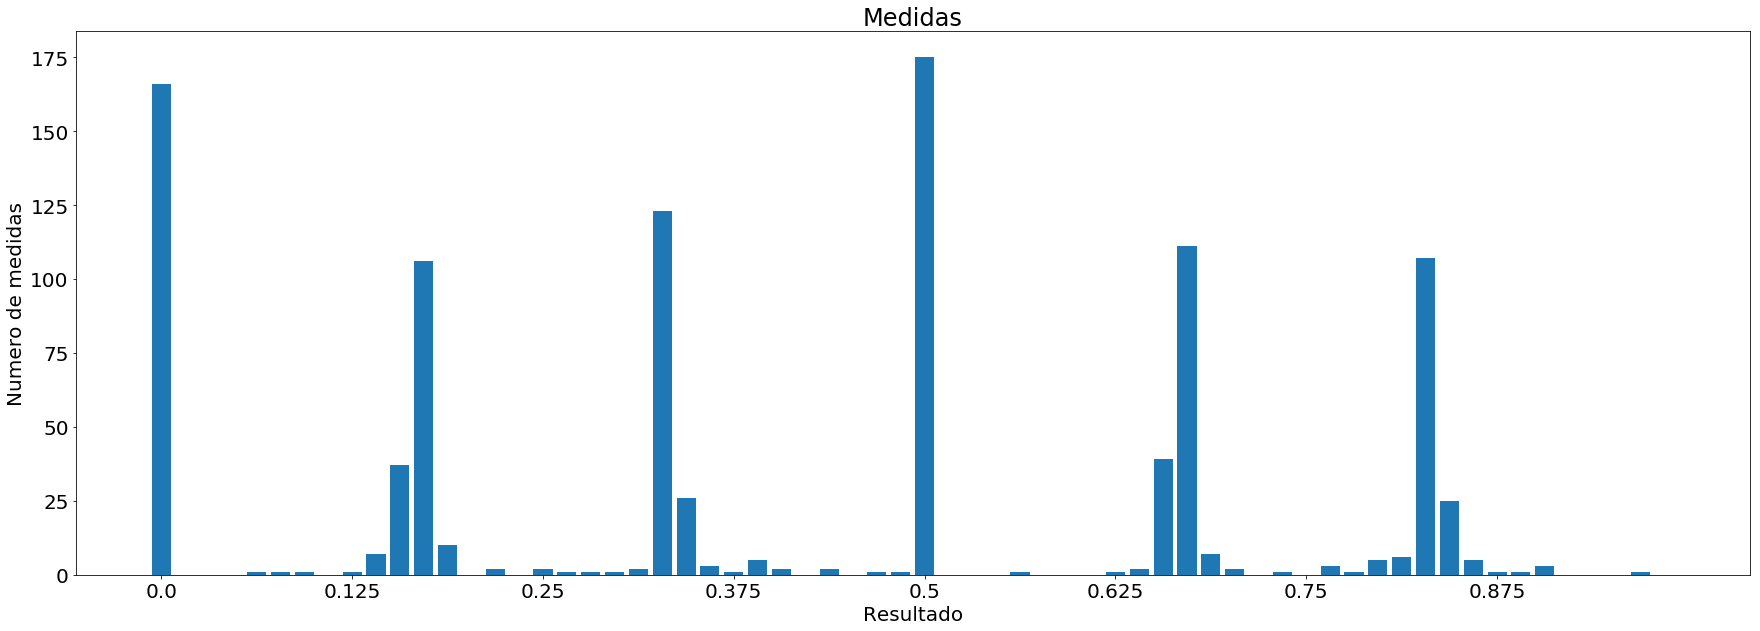
\includegraphics[scale=0.3]{relatorio-shor2.png}
\begin{figure}[h]
    \centering
    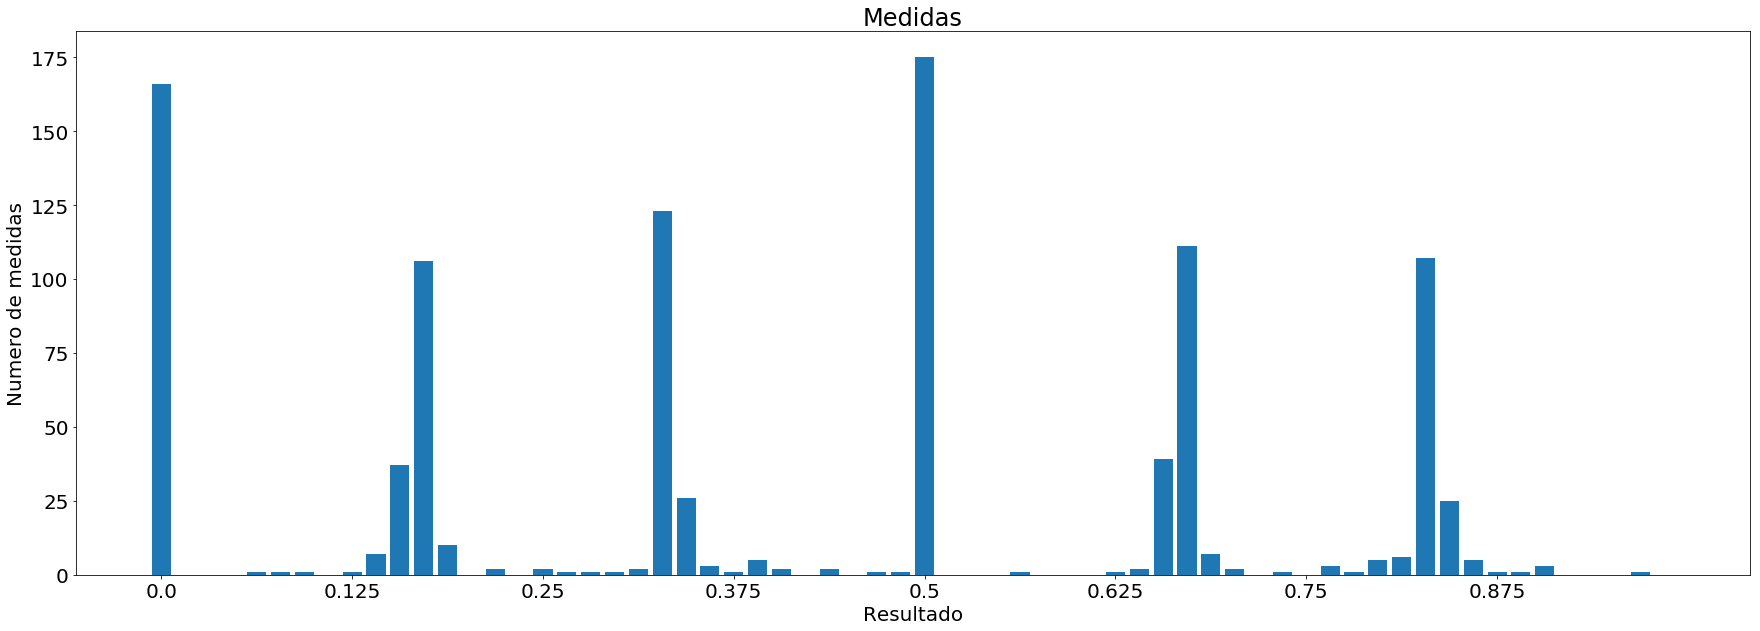
\includegraphics[width=1\textwidth]{relatorio-shor2.png}
    \caption{Histograma com valores obtidos para a aplicação do algoritmo de Shor com 12 qubits fatorando 21 com a=10}
    \label{fig:Shor1}
\end{figure}



% \textbf{Essa parte é para nos ajudar a fazer o relatório}


% \begin{enumerate}
% % \item Quais são os principais metas do projeto?


% \item O que foi realizado dentro essas metas (você deve fornecer informações para pelo menos uma das 4 categorias abaixo)?
% % \begin{enumerate}
% %     \item Principais Atividades
% %     \item Objetivos Específicos
% %      \item Resultados Significativos:
% %      \item Principais resultados ou outras conquistas
% %      \end{enumerate}
     


% % \item Que oportunidades de treinamento e desenvolvimento profissional o projeto ofereceu?



% \item Como os resultados foram divulgados às comunidades de interesse?
%     \begin{enumerate}
%      \item O que produzimos durante este periodo
%      \end{enumerate}
%      O caderno de Jupyter com as simulações foi disponibilizado no Github do aluno para ser utilizado por qualquer um.
     
% \item O que você planeja fazer durante o próximo período de relatório para atingir as metas?
% \end{enumerate}

\subsection{Implementação no computador Quântico}
Após a simulação do qubits foram utilizados os computadores quânticos disponibilizados pela IBM na IBM Quantum experience \cite{IBM2019IBMExperience}. Primeiro serão introduzidas novas portas quânticas que foram utilizadas e depois serão demonstrados os Algoritmos de Groover e Shor executados nessas máquinas. A linguagem utilizada para programar essas máquinas foi o Qiskit que é baseada em python. E que apresenta ferramentas para o desenvolvimento de circuitos para computadores quânticos e gera o QASM que é o Assembly para os computadores quânticos da IBM.

\subsubsection{Porta NOT}
A porta NOT é simples. Ela inverte as amplitudes dos valores $|0\rangle$ e $|1\rangle$ de um qubit. $X|\Psi\rangle=X(a|0\rangle+b|1\rangle)=b|0\rangle+a|1\rangle$ 
\begin{equation}
X=\left[ \begin{array}{cc} 0 & 1 \\ 1 & 0 \end{array}  \right] 
\end{equation}

\begin{figure}[h!]
    \centering
    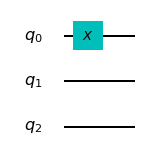
\includegraphics{Not_gate.png}
    
        \caption{Porta NOT}
    \label{fig:Xgate}
\end{figure}

Para usar uma porta no Qiskit. Declaramos um circuito e inserimos uma porta como a de NOT. A figura da porta é gerada pelo caderno Qiskit de Jupyter.
 \begin{minted}[mathescape, linenos]{python}
qc= QuantumCircuit(3)
qc.(0)
qc.draw()
\end{minted}[mathescape, linenos]{python}


\subsubsection{Porta de Toffoli}
A porta de Toffoli é uma porta CNOT controlada por dois qubits.

\begin{figure}[h!]
    \centering
    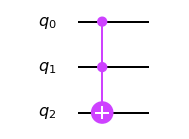
\includegraphics{Toffoli_gate.png}
    
        \caption{Porta de Toffoli}
    \label{fig:TFgate}
\end{figure}


\subsubsection{Porta SWAP e porta de Fredkin}
A porta SWAP troca dois qubits de lugar a de Fredkin é uma porta de SWAP controlada(CSWAP).

\begin{figure}[h]
    \centering
    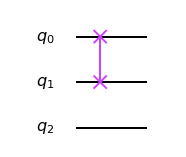
\includegraphics{porta_swap_simbolo.png}
    
        \caption{Porta SWAP}
    \label{fig:swapgate}
\end{figure}


\begin{figure}[h]
    \centering
    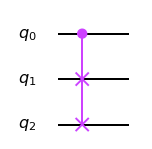
\includegraphics{fredkin_simbolo.png}
    
        \caption{Porta de Fredkin}
    \label{fig:frdgate}
\end{figure}

A Porta de SWAP e construída usando três portas CNOT alternadas.


\begin{figure}[h]
    \centering
    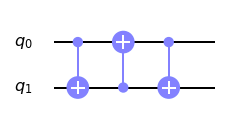
\includegraphics{porta_swap.png}
    
        \caption{Porta SWAP a partir de portas CNOT}
    \label{fig:swapconstr}
\end{figure}

A porta de Fredkin usa uma porta de Toffoli no lugar da CNOT do meio. Note que duas portas CNOT consecutivas revertem uma a outra e que uma porta de Toffoli com a sua entrada que não será trocada em 0 é o mesmo que se não houvesse nenhuma porta.

\begin{figure}[h]
    \centering
    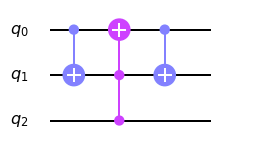
\includegraphics{porta_de_fredkin.png}
    \label{fig:Frdconstr}
    
        \caption{Porta de Fredkin a partir de portas CNOT e de Toffoli}
\end{figure}
\subsubsection{Portas  de mudança de fase e porta Y}

\begin{figure}[h!]
    \centering
    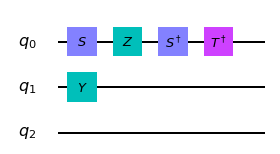
\includegraphics{portas_fase.png}
    
        \caption{Portas de mudança de fase e porta Y}
    \label{fig:TFgate}
\end{figure}

Embora no computador da IBM haja como usar uma porta de mudança de fase com valor de fase arbitrário. Usaremos as portas já configuradas com ângulos específicos.
\begin{equation}
     T=\left [ \begin{array}{cc}
         1 & 0\\
    0 & e^{i\pi/4 } 
    \end{array}\right ]
\end{equation}

 $ S=T^2 $,     $ \theta = \pi/2 $

$ Z=T^4 $,     $  \theta = \pi$

$ S^\dagger=T^6 $, $  \theta = -\pi/2$

$ T^\dagger=T^7 $, $  \theta = -\pi/4$

Assim como a porta Y que é uma combinação da porta X com a Z:
\begin{equation}
 Y=XZ=\left[\begin{array}{cc}
    0 & -i\\
    i & 0 
    \end{array}\right]
\end{equation}

\subsubsection{Algoritmo de Groover}
Para executar o algoritmo de Groover na máquina da IBM temos duas limitações principais. A primeira é que o algoritmo fica longo a medida que aumentamos o número de qubits. Isso porque precisamos repetir o oráculo e bloco de difusão de Groover que são pedaços do circuito $\pi/4\sqrt{2^N}$ vezes arredondado onde N é o número de qubits. O que já deixa o circuito longo para a máquina da IBM se usarmos 3 qubits.  E dependendo da máquina que utilizarmos como a IBM Q 14 Melbourne que tem mais qubits e portanto é mais suscetível a ruídos . Já será mais difícil distinguir a solução. 

A segunda limitação são as portas que podemos utilizar. Numa simulação com matrizes fica simples fazer uma porta que inverte a fase de apenas um elemento da base mas agora temos que implementar isso com outras portas quânticas fundamentais. Felizmente para três qubits podemos usar uma porta Z controlada por dois qubits que pode ser feita com uma porta de Toffoli e duas de Hardamard nas entradas do qubit que será negado. Essa porta inverte a fase do componente $|111\rangle$ apenas. Para usar em outros elementos podemos colocar portas NOT na entrada e saída dessa porta para que mude a fase de outra combinação de qubits. 




\begin{figure}[h!]
    \centering
    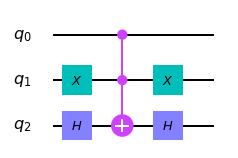
\includegraphics{oraculo101.png}
        \caption{Oráculo quântico para o valor 5 = |101\rangle. Note nas portas X no qubit que é 0}
    \label{fig:orac101}
\end{figure}


Código do algoritmo de Groover em qiskit:
\begin{minted}[mathescape, linenos]{python}
#Hadamards em todos os qubits
hadamards=QuantumCircuit(3)
#Inicializa todos os qubits em superposicao
hadamards.h(0)
hadamards.h(1)
hadamards.h(2)
hadamards.draw()

#----------------------------------

resposta=5

#oraculo quantico ###########################################
oracle=QuantumCircuit(3)
#coloca portas X antes dos bits 0 da resposta
if(resposta % 2 == 0):
    oracle.x(0)
if((resposta % 4) //2 == 0):
    oracle.x(1)
if( (resposta % 8) //4 == 0):
    oracle.x(2)

#porta Z em 2 controlada por 0 e 1
oracle.h(2)
oracle.ccx(0,1,2)
oracle.h(2)

#coloca portas X depois dos bits 0 da resposta
if(resposta % 2 == 0):
    oracle.x(0)
if((resposta % 4) //2 == 0):
    oracle.x(1)
if( (resposta % 8) //4 == 0):
    oracle.x(2)
oracle.draw()
#--------------------------------------
#Operador de difusão de groover
difusao=QuantumCircuit(3)
#hadamards
difusao=difusao+hadamards

#portas x para o estado |000> 
difusao.x(0)
difusao.x(1)
difusao.x(2)

#porta Z controlada 
difusao.h(2)
difusao.ccx(0,1,2)
difusao.h(2)

difusao.x(0)
difusao.x(1)
difusao.x(2)

#hadamards
difusao=difusao+hadamards

difusao.draw()

#----------------------------------
#parte de medida do circuito
mdir=QuantumCircuit(3,3)
grvc=QuantumCircuit(3)
mdir.measure(range(3),range(3)) #circuito para a medicao dos qubits

#oraculo e o operador de difusao sao repetidos 2 vezes
grvc=hadamards+oracle+difusao+oracle+difusao+mdir

grvc.draw()

\end{minted}[mathescape, linenos]{python}


\begin{figure}[h!]
    \centering
    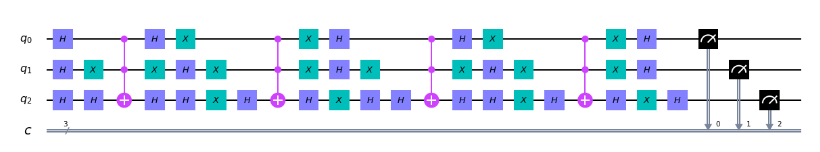
\includegraphics[width=1\textwidth]{groover3qubits.png}
        \caption{Circuito de Groover para três qubits}
    \label{fig:orac101}
\end{figure}

O programa foi executado duas vezes. A primeira foi uma simulação. Logo apresenta o resultado sem ruídos. Código para simular o circuito:

\begin{minted}[mathescape, linenos]{python}

#simulacao de um computador quantico
backend_sim = Aer.get_backend('qasm_simulator')
job_sim = execute(grvc, backend_sim, shots=1024)
result_sim = job_sim.result()
plot_histogram(result_sim.get_counts(grvc))
\end{minted}[mathescape, linenos]{python}



\begin{figure}[h!]
    \centering
    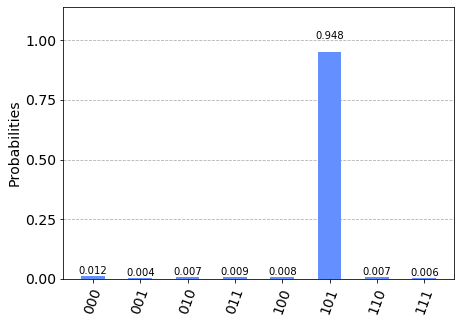
\includegraphics[width=1\textwidth]{grooversimu.png}
        \caption{Resultado da simulação de QASM num computador clássico da IBM}
    \label{fig:resultadogrooversimu}
\end{figure}

A segunda é a execução no computador quântico. Podemos notar como aparecem mais das outras medidas que não são o resultado:


Código para executar o circuito na máquina quântica da IBM:
\begin{minted}[mathescape, linenos]{python}
#executa o circuito em um computador quantico real
from qiskit.tools.monitor import job_monitor
backend = provider.get_backend('ibmqx2')

job = execute(grvc, backend=backend, shots=4096)
job_monitor(job)

##################################
resultado_comp = job.result()
plot_histogram(resultado_comp.get_counts(grvc))

\end{minted}[mathescape, linenos]{python}


\begin{figure}[h!]
    \centering
    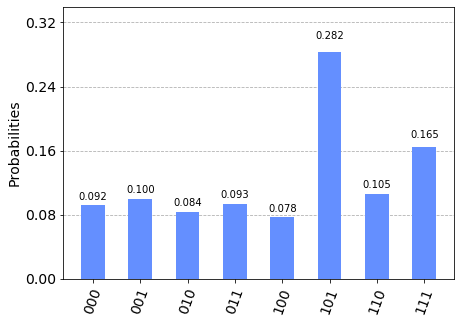
\includegraphics[width=1\textwidth]{groovercq.png}
        \caption{Resultado do programa com algoritmo de Grover rodado no computador quântico ibmqx2}
    \label{fig:groovercq}
\end{figure}

\subsubsection{Algoritmo de Shor}
No algoritmo de Shor a maior limitação para a implementação em um computador quântico real é a porta quântica que faz a multiplicação por $a^x\,mod\,C$. Já que temos que implementá-la através de outras portas mais fundamentais e não diretamente através da matriz como na simulação. A transformada de Fourier Quântica é simples de implementar assim como a superposição inicial. 

Primeiro implementei um circuito mais simples com 5 qubits usando $C=15$ e $a=4$ que têm um período de apenas 2 o que permite encolher bastante o circuito.

Para fazer o multiplicador por $a^x\, mod\, 15=4^x\, mod\, 15$. Dividimos ele em duas partes: $4^1\, mod\, 15$ controlado pelo qubit de $x$ menos significativo e $4^2\, mod\, 15$ controlado pelo mais significativo. Assim se o qubit de $x$ menos significativo for 1 multiplicamos $f$ por $4\,mod\,15$ e o mesmo para o mais. Obtendo assim $4^{x_0+x_1}\, mod\, 15$. Como $4^2\,mod\,15=16\,mod\,15=1$ precisamos fazer apenas o do bit menos significativo. Para multiplicar o número 1 por 4 sempre que o qubit menos significativo de $x$ for 1 basta usar uma porta CNOT que zera a porta com 1 do digito menos significativo com peso 1 e uma que seta o qubit com peso 4.

\begin{minted}[mathescape, linenos]{python}

hadamards=QuantumCircuit(5)
#Inicializa os qubits do registradores de L em superposicao
hadamards.h(3)
hadamards.h(4)
hadamards.draw()
#######################################
#multiplicador
mult=QuantumCircuit(5)
mult.x(0)#inicializa o registrador f em 1

mult.cx(3,2)#seta q2(f2) se q3(x0) for um
mult.cx(3,0)#zera q0(f0) se q3(x0) for um
mult.draw()
################################
#transformada de Fourier quantica
from math import pi
iqft=QuantumCircuit(5)
iqft.h(4)
iqft.crz(pi/2, 4, 3)
iqft.h(3)
iqft.draw()

###################################
#parte de medida

mdir=QuantumCircuit(5,2)
shor=QuantumCircuit(5)
mdir.measure([3, 4],[1,0]) #circuito para a medicao dos qubits

#oraculo e o operador de difusoa sao repetidos 2 vezes
shor=hadamards+mult+iqft+mdir

shor.draw()

\end{minted}[mathescape, linenos]{python}

Para rodar o circuito usamos o mesmo código do algoritmo de Groover só que agora no computador quântico \textbf{ibmq 16 melbourne}.


\begin{figure}[h!]
    \centering
    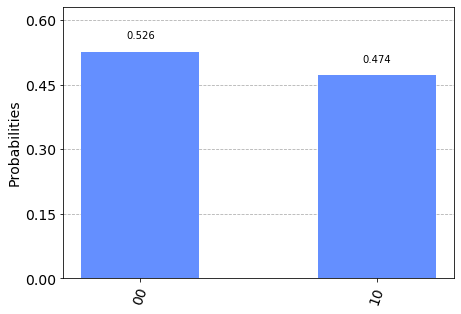
\includegraphics[width=1\textwidth]{shora4simu.png}
        \caption{Resultado da simulação do Algoritmo de Shor com C=15 a=4}
    \label{fig:shora4simu}
\end{figure}


\begin{figure}[h!]
    \centering
    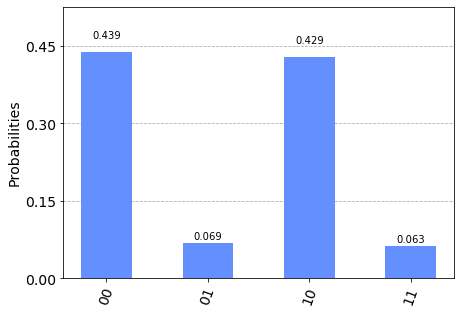
\includegraphics[width=1\textwidth]{shora4cq.png}
        \caption{Resultado da execução do Algoritmo de Shor com C=15 a=4 no \textbf{ibmq 16 melbourne}}
    \label{fig:groovercq}
\end{figure}


\begin{figure}[h!]
    \centering
    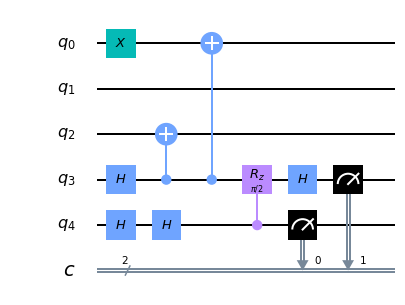
\includegraphics[width=1\textwidth]{shora4draw.png}
        \caption{Circuito do Algoritmo de Shor com C=15 a=4}
    \label{fig:groovercq}
\end{figure}

Agora executamos o algoritmo com a=2 o que vai requerer 6 qubits.
O novo multiplicador é assim: $a^x\, mod\, 15=2^x\, mod\, 15$. Dividimos ele em 3 partes: $2^1\, mod\, 15$ controlado pelo qubit de $x$ menos significativo, $2^2\, mod\, 15$ controlado pelo qubit do meio e $2^4\, mod\, 15$ controlado pelo mais significativo. Assim se o qubit de $x$ menos significativo for 1 multiplicamos $f$ por $2\,mod\,15$ e o mesmo para os outros. Obtendo assim $4^{x_0+x_1+x_2}\, mod\, 15$. Como $2^4\,mod\,15=16\,mod\,15=1$ precisamos fazer apenas o do meio e o do qubit menos significativo. Para multiplicar um número por 2 módulo 15 vamos usar três portas de Fredkin. 
Para números binários, a multiplicação por dois é um deslocamento para a esquerda. Como fazemos o módulo 15 do valor também note que os números dão a volta pela esquerda de volta a direta, como uma rotação. Para fazer esse deslocamento usamos portas de Fredkin para fazer SWAPs controlados nos qubits de $f$. Para multiplicar por $2^2=4$ o circuito vai funcionar de maneira semelhante. Só que com um deslocamento de dois qubits.


\begin{figure}[h!]
    \centering
    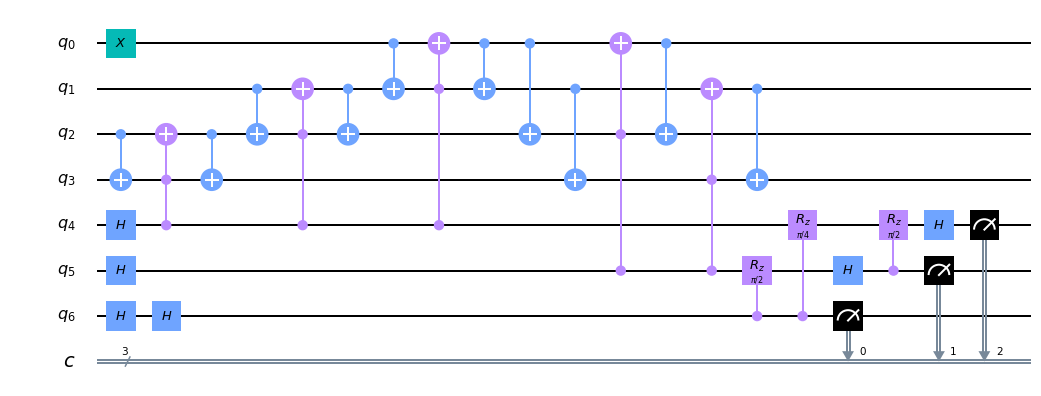
\includegraphics[width=1\textwidth]{shora2draw.png}
        \caption{Circuito do Algoritmo de Shor com C=15 a=2}
    \label{fig:groovercq}
\end{figure}

\begin{figure}[h!]
    \centering
    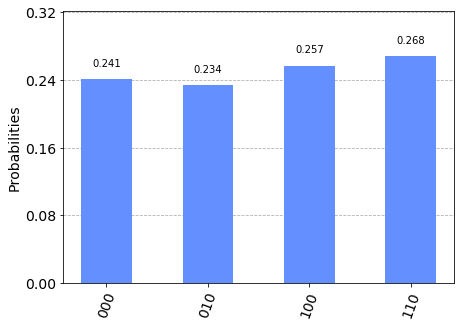
\includegraphics[width=1\textwidth]{shora2simu.png}
        \caption{Resultado da simulação do Algoritmo de Shor com C=15 a=2}
    \label{fig:shora4simu}
\end{figure}


\begin{figure}[h!]
    \centering
    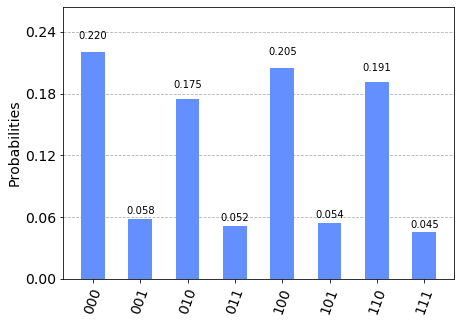
\includegraphics[width=1\textwidth]{shora2cq.png}
        \caption{Resultado da execução do Algoritmo de Shor com C=15 a=2 no \textbf{ibmq 16 melbourne}}
    \label{fig:groovercq}
\end{figure}



\begin{minted}[mathescape, linenos]{python}

hadamards=QuantumCircuit(7)
#Inicializa os qubits do registradores de L em superposicao
hadamards.h(4)
hadamards.h(5)
hadamards.h(6)
hadamards.x(0)#inicializa o registrador f em 1
hadamards.draw()
##########################
#multiplica f por 2^1 mod 15
mult21=QuantumCircuit(7)

#fredkin controlado por q4(x0) em q2(f2) e q3(f3)
mult21.cx(2,3)
mult21.ccx(4,3,2)
mult21.cx(2,3)

mult21.cx (1,2)
mult21.ccx (4,2,1)
mult21.cx (1,2)

mult21.cx (0,1)
mult21.ccx (4,1,0)
mult21.cx (0,1)

mult21.draw()
################################
#multiplica f por 2^2 mod 15
mult22=QuantumCircuit(7)

#fredkin controlado por q5(x1) em q0(f0) e q2(f2)
mult22.cx (0,2)
mult22.ccx (5,2,0)
mult22.cx (0,2)

mult22.cx (1,3)
mult22.ccx (5,3,1)
mult22.cx (1,3)

mult22.draw()
##################################
#IQFT em x

from math import pi
iqft=QuantumCircuit(7)
iqft.h(6)
iqft.crz(pi/2, 6, 5)
iqft.crz(pi/4, 6, 4)

iqft.h(5)
iqft.crz(pi/2,5, 4)

iqft.h(4)
iqft.draw()
 
 ##################################
 #medida
 
mdir=QuantumCircuit(7,3)
shor=QuantumCircuit(5)
mdir.measure([4, 5, 6],[2,1,0]) #circuito para a medicao dos qubits(bits de medida ja trocados)

#oraculo e o operador de difusoa sao repetidos 2 vezes
shor=hadamards+mult21+mult22+iqft+mdir

shor.draw()

\end{minted}[mathescape, linenos]{python}

\section{Conclusões}
Ao longo da realização do projeto, tivemos contato com diversas áreas do conhecimento, relacionado principalmente com a computação quântica. Dentro da própria física, conceitos como a superposição quântica e fases da função de onda foram revisitados para melhor compreensão, como também um estudo aprofundado dos algorítimos de Groover de busca e Shor de fatoração de números inteiros. Desenvolvemos as implementações destes algorítimos em Python e fizemos simulações para diversas situações. Utilizando os computadores quânticos da IBM implementamos os algoritmos de Shor e Groover e comparamos os resultados com nossa simulação clássica, obtendo resultados similares.

Em conclusão, desenvolvemos com sucesso todo o processo de implementação, simulação e análise de algorítimos quânticos, e fizemos um estudo de tópicos avançados de mecânica quântica com enfase em computação quântica.


\newpage
%\section{Conclusão e trabalhos para próximo período}

%No próximo semestre vamos utilizar o computador quântico disponibilizado em nuvem pela IBM para executar o algoritmo de Shor e de Groover. Para isso será necessário aprender a programar em Qiskit, a linguagem de programação de computadores quânticos da IBM. Assim como a lidar com as limitações de um computador real onde há ruídos e as portas quânticas são mais limitadas.




\singlespacing %Para um espaçamento simples
\setlength{\bibsep}{0.0pt}
\bibliography{references.bib}
\printbibliography

%\marginpar{Coloca anotações na margem}

\end{document}